\documentclass[aspectratio=169]{beamer} % 16:9 aspect ratio for modern screen
% \documentclass[handout]{beamer}
% \documentclass[notes=only]{beamer}

% Theme settings
\usetheme[progressbar=foot]{metropolis} % Minimalist theme
\metroset{progressbar=frametitle} % Progress bar soll nur folien mit titel berücksichtigtigen?
\setbeamercolor{background canvas}{bg=white} % White background color

\makeatletter
    \setlength{\metropolis@progressinheadfoot@linewidth}{1.5pt}
\makeatother


\usefonttheme{professionalfonts} % Font theme

% Packages
\usepackage[T1]{fontenc}   % Font encoding
\usepackage[ngerman]{babel} % German language
\usepackage[sfdefault]{FiraSans} % For FiraSans font
\usepackage[backend=biber, style=authoryear-comp
, sorting=nyt]{biblatex} % For bibliography
\usepackage{csquotes} % Recommended for biblatex with babel/polyglossia
\usepackage{textgreek} % Greek letters in text mode (aus references von Citavi)
\usepackage{tikz}          % For drawing graphics
\usepackage{animate} % Für Animation

\usepackage{graphicx}       % For including images
\usepackage{amsmath, amssymb} % For math symbol

% \usepackage{media9} % For embedding videos

\usepackage[labelformat=empty]{caption}


% Bibliography settings
\addbibresource{references.bib} % Path to the bibliography file

% custom Citation commands
\DeclareCiteCommand{\citeauthortitle}
  {\usebibmacro{prenote}}
  {\usebibmacro{citeindex}%
   \printnames{labelname}%
   \setunit{\space\textendash\space}
   \printfield{title}}
  {\multicitedelim}
  {\usebibmacro{postnote}}

  \DeclareCiteCommand{\citeauthortitleurl}
  {\usebibmacro{prenote}}
  {\usebibmacro{citeindex}%
   \printnames{labelname}%
   \setunit{\space\textendash\space}
   \printfield{title}%
   \setunit{\addsemicolon\space}
   \printfield{url}}
  {\multicitedelim}
  {\usebibmacro{postnote}}

\DeclareCiteCommand{\parenciteauthortitle}
  {\usebibmacro{prenote}}
  {\bibopenparen\usebibmacro{citeindex}%
   \printnames{labelname}%
   \setunit{\space\textendash\space}% <- Hier wird das Trennzeichen ":" hinzugefügt
   \printfield{title}\bibcloseparen}
  {\multicitedelim}
  {\usebibmacro{postnote}}

\makeatletter
\renewcommand\footnotesize{\tiny}
\makeatother

\newcommand{\figcite}[1]{\\[-3mm]{\tiny Quelle: \cite{#1}}}
\newcommand{\figciteweb}[1]{\\[-3mm]{\tiny aus: \citeauthortitle{#1}}}
\newcommand{\figciteweburl}[1]{\\[-3mm]{\tiny aus: \citeauthortitleurl{#1}}}
  
\mode<handout>{
    \AtBeginSection[]{} % In Handout-Version keine Section-Folie erzeugen
}

% Title page settings
\title{Second- \& Third-Harmonic Generation}
\subtitle{Frequenzverdopplung in der nichtlinearen Optik}
\author{Florian Marius Adamczyk}
\date{07.07.2025}
\institute{Justus-Liebig-Universität Gießen \\ M.Sc. Modul \textbf{Spektroskopie} bei \textbf{PD Dr. Arash Rahimi-Iman, Dipl.-Ing.}\\ }
\titlegraphic{\vspace{-1cm}
\includegraphics[height=1.2cm]{Images/jlu_logo.jpg}}

\begin{document}

    % Black slide
    \begin{frame}<handout:0>[plain, noframenumbering]
        \begin{tikzpicture}[remember picture, overlay]
          \fill[black] (current page.south west) rectangle (current page.north east);
        \end{tikzpicture}
        \pause
        .
        \pause
        \centering
        \only<3>{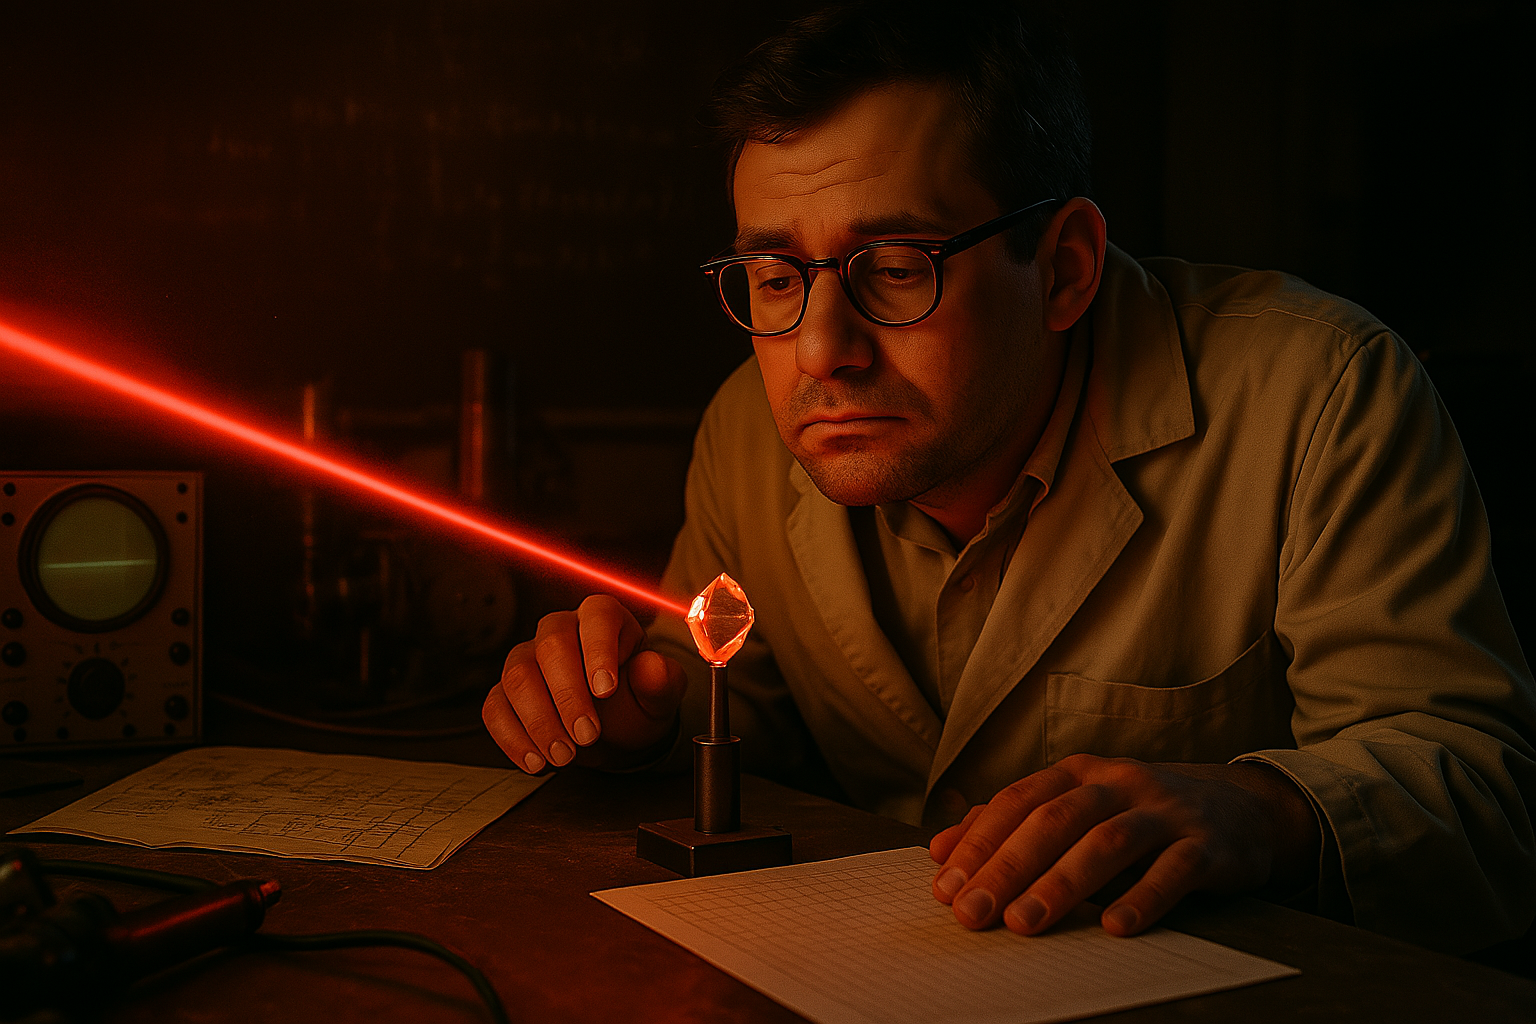
\includegraphics[width=0.9\textwidth]{Images/Copilot_20250706_224005.png}}
        \only<4>{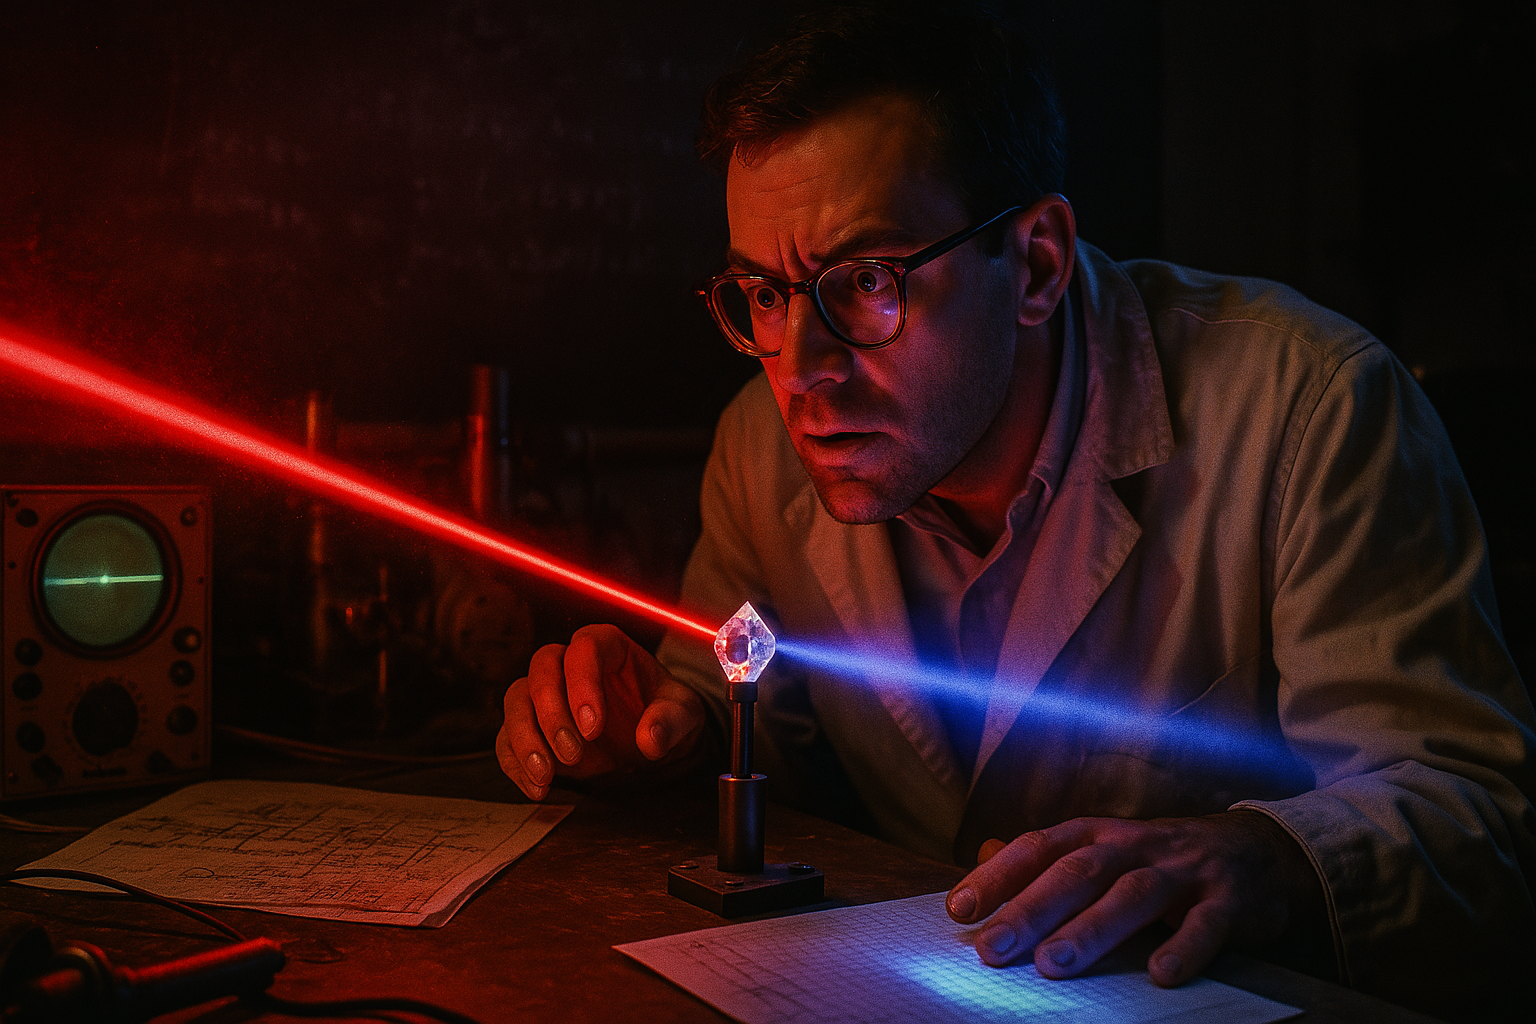
\includegraphics[width=0.9\textwidth]{Images/Copilot_20250706_215901.png}}
        \\ \tiny \textcolor{gray}{von: \citetitle{Copilot.2025} -- \citefield{Copilot.2025}{note}}
        \note{1961 beobachteten der Physiker Peter Franken und seine Mitarbeiter an der University of Michigan einen merkwürdigen Effekt: Bei der Bestrahlung eines Quarzkristalls mit einem der ersten Rubinlaser bestand das transmittierte Licht nicht nur aus Strahlung der Laserwellenlänge 694 nm, sondern es trat auch UV-Licht der halben Wellenlänge 347 nm aus. Das war die erste Beobachtung eines nichtlinearen Effektes, der Frequenzverdopplung,[2] und gilt als die Geburtsstunde der nichtlinearen Optik.}
    \end{frame}
   

    % % Appetizer Slide
    % \begin{frame}<handout:0>[noframenumbering, plain]{Appetizer}
    %     \centering
    %     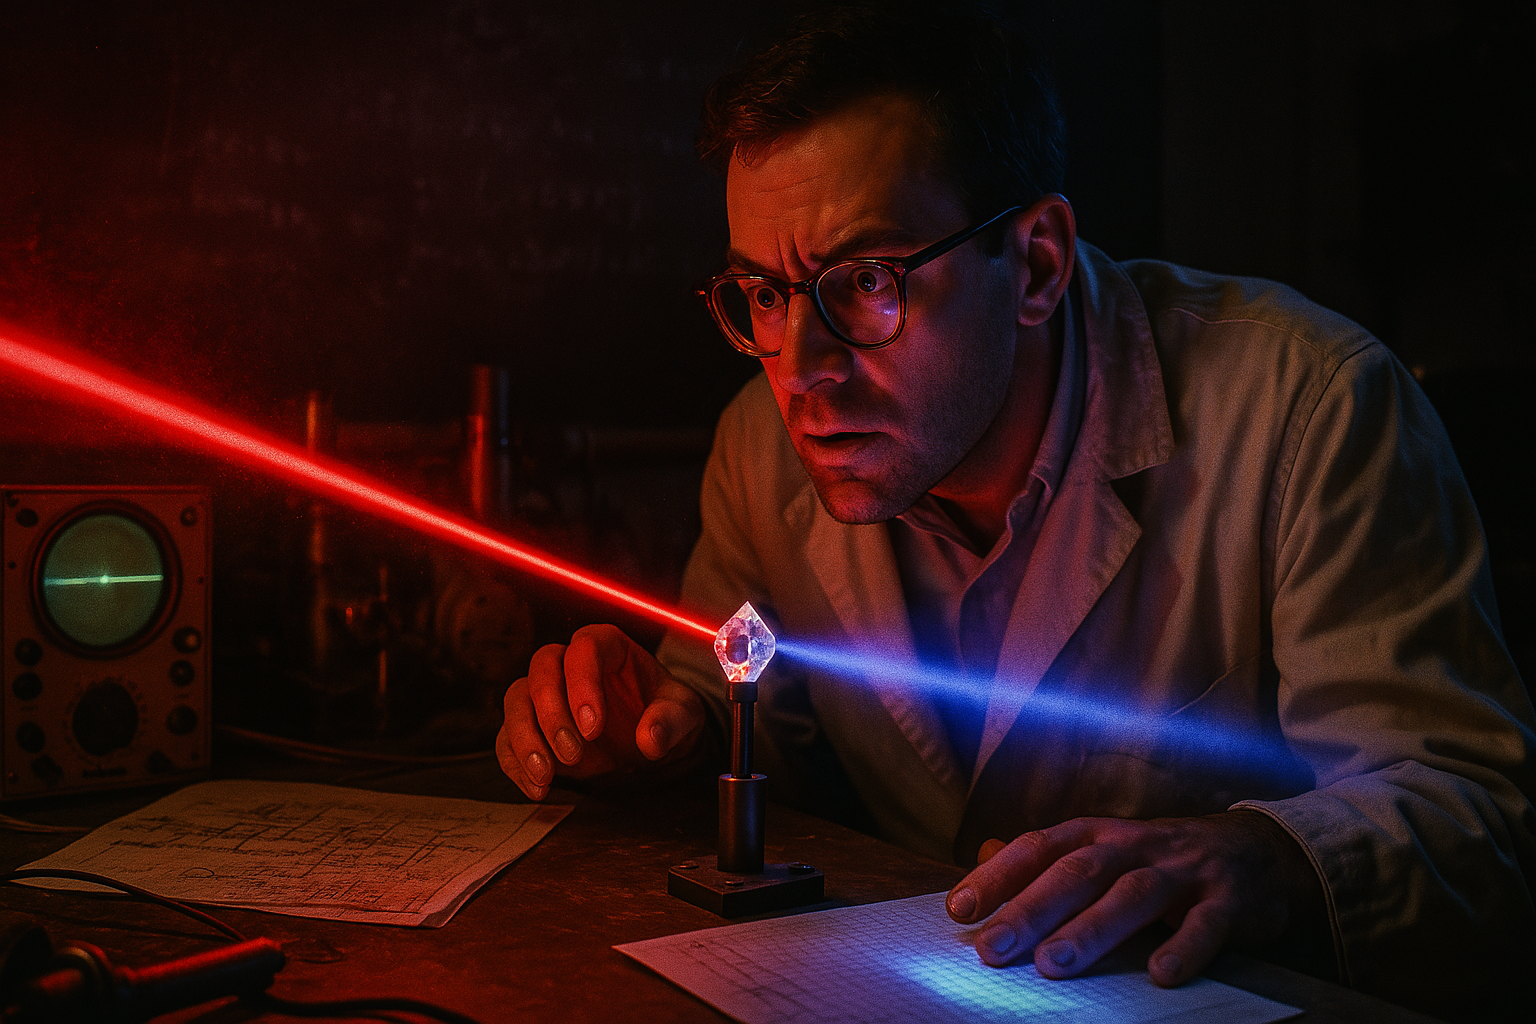
\includegraphics[width=\textwidth, height=0.9\textheight, keepaspectratio]{Images/Copilot_20250706_215901.png}
    %     \figciteweburl{Copilot.2025}
    %     % \vspace{0.5cm}
    %     % \begin{quote}
    %     %{Stellen Sie sich vor, ...}
    %     % \end{quote}
    % \end{frame}

    % Title Slide
    \begin{frame}[noframenumbering, plain]
        \vspace*{-0.6cm}
        \titlepage
        \vspace*{-1.6cm}
    \end{frame}
    
    % Table of Contents
    \begin{frame}<handout:0>{Gliederung} % Handout ausgeschaltet!!
      \setcounter{page}{1}      
        \tableofcontents
    \end{frame}
      \note{
        In dieser Präsentation beginnen wir mit den Grundlagen der nichtlinearen Optik. 
        Anschließend erkläre ich die Prinzipien der Frequenzverdopplung (SHG) und -verdreifachung (THG), 
        bevor wir auf das wichtige Konzept der Phasenanpassung eingehen. 
        Danach stelle ich einen typischen experimentellen Aufbau vor und zeige Beispiele sowie Anwendungen. 
        Am Ende folgt eine kurze Zusammenfassung. 
        Ziel ist es, dass Sie zunächst die grundlegenden Konzepte verstehen und dann nachvollziehen können, wie SHG und THG funktionieren.
      }
    
    % presentation slides
  
    \section{Einführung in die nichtlineare Optik}

\begin{frame}{Was ist nichtlineare Optik?}
  % Breite, niedrige Grafik oben
  \begin{center}
    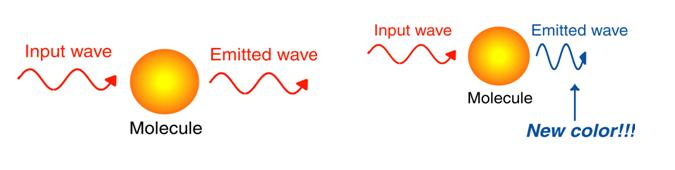
\includegraphics[width=0.6\textwidth]{Images/Fig.1 optics.jpeg}\\
    {\tiny Fig. 1: Linear (links) und nichtlineare (rechts) Wechselwirkung von Licht und Materie. Quelle: \cite{Science20NonlinearOptics2014}}
  \end{center}
  \vspace{0.2cm}
  \begin{columns}[T,onlytextwidth]
    \column{0.48\textwidth}
      \begin{itemize}
        \item \textbf{Lineare Optik:} $P \propto E$
        \pause
        \item Materialantwort ist direkt proportional zum elektrischen Feld
        \item Gilt für alltägliche Lichtquellen (Sonne, Lampe)
      \end{itemize}
    \column{0.48\textwidth}
      \begin{itemize}
        \item \textbf{Nichtlineare Optik:} $P = \varepsilon_0(\chi^{(1)}E + \chi^{(2)}E^2 + \chi^{(3)}E^3 + \dots)$
        \pause
        \item Zusätzliche Terme treten erst bei sehr hohen Intensitäten auf (starke Laser!)
      \end{itemize}
  \end{columns}
  \note{
    Die Grafik oben zeigt links die lineare, rechts die nichtlineare Antwort eines Mediums auf einfallendes Licht.\newline
    In der linearen Optik ist die Polarisation $P$ proportional zum Feld $E$. Erst bei sehr hohen Intensitäten (typisch: starke Laser) treten nichtlineare Terme auf.\newline
    Diese führen dazu, dass das Material neue Frequenzen erzeugt – z.B. die doppelte oder dreifache Frequenz des eingestrahlten Lichts.\newline
    Das ist die Grundlage für Second Harmonic Generation (SHG) und Third Harmonic Generation (THG).\newline
    Im Alltag bleibt die Optik fast immer linear, nichtlineare Effekte sind selten und erfordern spezielle Bedingungen.
  }
\end{frame}

\section{Harmonische Generation}

% --- Folie 5: Zweitharmonische Generation (SHG) – Prinzip ---

\begin{frame}{Zweitharmonische Generation (SHG): Prinzip}
  \begin{columns}[T,onlytextwidth]
    \column{0.55\textwidth}
      \begin{itemize}
        \item Einfallende elektromagnetische Welle übt Kraft auf Elektronen (Dipolschwingung)
        \pause
        \item Elektrisches Feld $E(t)$ versetzt Elektronen in periodische Bewegung
        \item Bewegung erzeugt zeitabhängige Polarisation $P(t)$ {\tiny (\citetitle{WikipediaNonlinearOpticalProcess2006})}
        \pause
        \item Voraussetzung für SHG: Material nicht-zentrosymmetrisch ($\chi^{(2)} \neq 0$)
        \item $P^{(2)}(2\omega) = \varepsilon_0 \chi^{(2)} E(\omega)^2$
        \item $E(2\omega) \propto \chi^{(2)} [E(\omega)]^2$
        % \item Energieerhaltung: $2\hbar\omega = \hbar(2\omega)$
      \end{itemize}
    \column{0.43\textwidth}
      %hier gif
      \begin{center}
      \animategraphics[autoplay,loop,width=0.95\columnwidth]{20}{Images/Electron_asymmetric_motion_animation/frame}{001}{060}
      \\[-1mm]{\tiny Elektronenbewegung im anharmonischen Potential: Neben der Grundfrequenz entstehen neue Frequenzen (Fourierpfeile: blau\:=\:linear, grün\:=\:SHG, rot\:=\:optische Rektoifikation). \figciteweburl{Sbyrnes3212014}}
      \end{center}
  \end{columns}
  \note{
    Bei der SHG verschmelzen zwei Photonen der Frequenz $\omega$ zu einem Photon mit $2\omega$.\newline
    Das funktioniert nur in Materialien ohne Inversionssymmetrie, weil nur dann $\chi^{(2)}$ ungleich null ist.\newline
    Formel: Die induzierte Polarisationskomponente bei 2ω ist $P^{(2)}(2\omega)=\varepsilon_0\chi^{(2)}E(\omega)E(\omega)$, daraus folgt für das elektrische Feld $E(2\omega)\propto \chi^{(2)}[E(\omega)]^2$. (Folie: Grafik oder Formel zeigen.)\newline
    Die Elektronenbewegung im anharmonischen Potential ist nicht mehr sinusförmig – dadurch entstehen neue Frequenzen (siehe Fourierpfeile in der Animation).\newline
    Die Formel $P^{(2)}(2\omega) = \varepsilon_0 \chi^{(2)} E(\omega)^2$ beschreibt die Polarisationskomponente bei $2\omega$.\newline
    Energieerhaltung: Zwei Photonen werden zu einem mit doppelter Energie.
  }
\end{frame}

\begin{frame}{Materialantwort: Wann tritt Nichtlinearität auf?}
  \begin{columns}[T,onlytextwidth]
    \column{0.38\textwidth}
      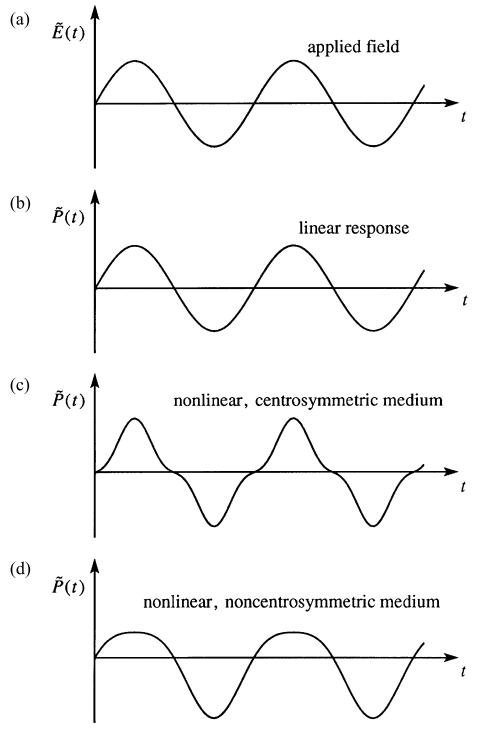
\includegraphics[height=0.8\textheight]{Images/Nonlinear response.png}
      {\tiny \figcite{Boyd2020}: \citetitle{Boyd2020}}
    \column{0.6\textwidth}
      \begin{itemize}
        \item Antwort eines Mediums auf sinusförmiges Feld
        \pause
        \item Bei nichtlinearen Bedingungen: Verzerrte Schwingung $\rightarrow$ neue Frequenzen
        \item \textbf{Symmetrie entscheidend:}
          \begin{itemize}
            \item Zentrosymmetrisch: $\chi^{(2)} = 0$ (z.B. Glas, Wasser)
            \item Nicht-zentrosymmetrisch: $\chi^{(2)} \neq 0$ (z.B. viele Kristalle)
          \end{itemize}
      \end{itemize}
  \end{columns}
  \note{
    Die Grafik zeigt, wie verschiedene Materialien auf ein sinusförmiges elektrisches Feld reagieren.\newline
    Nur Materialien ohne Inversionssymmetrie (z.B. viele Kristalle) zeigen eine starke nichtlineare Antwort ($\chi^{(2)} \neq 0$).\newline
    In zentrosymmetrischen Medien verschwindet $\chi^{(2)}$, sodass nur Effekte dritter Ordnung ($\chi^{(3)}$) wie THG möglich sind.\newline
    Die verzerrte Schwingung im rechten Teil der Grafik steht für die Entstehung neuer Frequenzen durch Nichtlinearität.
  }
\end{frame}

% --- Folie 6: Zweitharmonische Generation (SHG) – Beispiele & Bedingungen ---

\begin{frame}{Zweitharmonische Generation (SHG): Beispiele \& Bedingungen}
  \begin{columns}[T,onlytextwidth]
    \column{0.55\textwidth}
      \begin{itemize}
        \item Benötigt starke, gepulste Laser (z.B. Nd:YAG 1064 nm $\rightarrow$ 532 nm grün)
        \item Effizienz oft gering, exakte Ausrichtung nötig
        \item SHG historisch erstmals 1961 mit Rubinlaser beobachtet (Franken)
        \item \textbf{Praxis:} Quadratische Abhängigkeit der SHG-Intensität von der Eingangsleistung
      \end{itemize}
    \column{0.43\textwidth}
      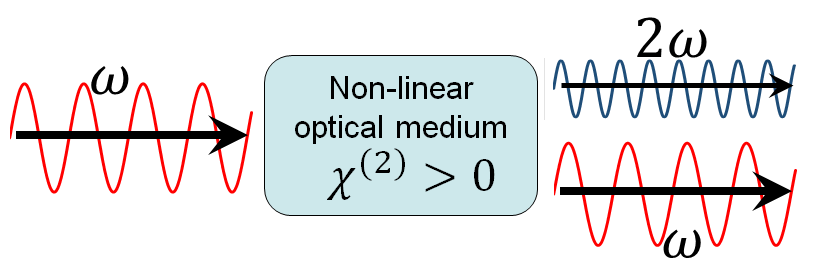
\includegraphics[width=0.95\textwidth]{Images/Schematic_of_the_SHG_conversion_of_an_excited_wave_in_a_non-linear_medium.png}\\
      {\tiny Schematische Darstellung: Einfallende Welle erzeugt zweite Harmonische im nichtlinearen Medium. \figcite{BPAegirsson2017}}
      \pause
      \begin{itemize}
        \item Typische Kristalle: 
          \begin{itemize}
            \item BBO (Beta-Bariumborat)
            \item KTP (Kaliumtitanylphosphat)
            \item KDP (Kaliumdihydrogenphosphat)
            \item LBO (Lithiumtriborat)
          \end{itemize}
      \end{itemize}
  \end{columns}
  \note{
    Für effiziente SHG braucht man starke, meist gepulste Laser und spezielle Kristalle ohne Inversionssymmetrie.\newline
    Typische Materialien sind BBO, KTP, KDP oder LBO.\newline
    Die Effizienz ist oft gering, daher ist eine exakte Ausrichtung und Phasenanpassung wichtig.\newline
    Praktisch wird z.B. aus einem 1064 nm Nd:YAG-Laser durch SHG ein 532 nm grüner Strahl erzeugt.\newline
    Die schematische Grafik zeigt, wie im Kristall aus der Grundwelle die zweite Harmonische entsteht.
  }
\end{frame}


\begin{frame}{Energieerhaltung und Photonenprozesse}
  \begin{columns}[T,onlytextwidth]
    \column{0.38\textwidth}
      % SHG & THG Formeln
      \vspace{1.6cm}
      \begin{itemize}
        \item \textbf{SHG:} $2\,\hbar\omega \rightarrow \hbar(2\omega)$
        \pause
        \item \textbf{THG:} $3\,\hbar\omega \rightarrow \hbar(3\omega)$
        \item \textbf{Energieerhaltung:} $n\,\hbar\omega = \hbar(n\omega)$
      \end{itemize}
    \column{0.6\textwidth}
      \centering
      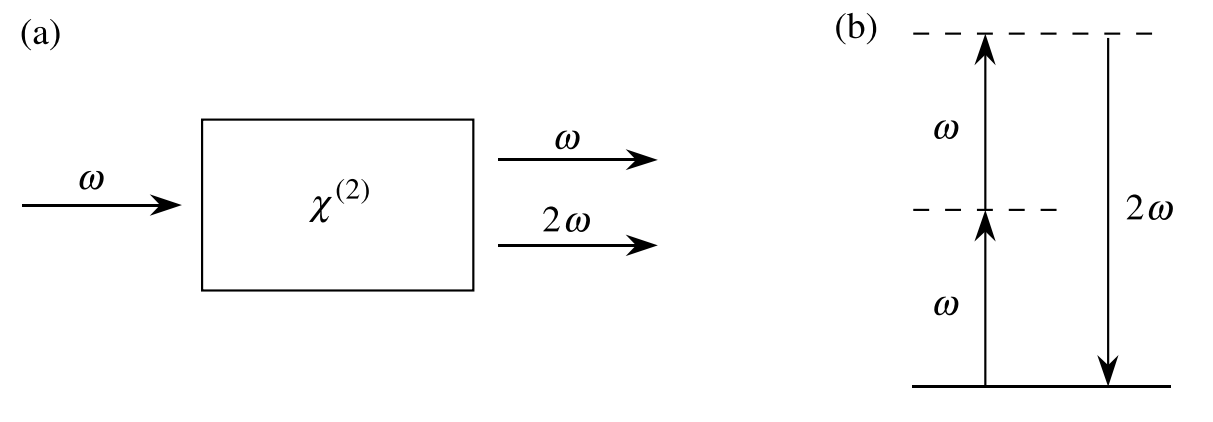
\includegraphics[width=0.98\textwidth]{Images/shg.png}\\
      \small SHG: $\omega \rightarrow 2\omega$
      {\figcite{Boyd2020}}
  \end{columns}

  \vspace{0.2cm}

  \begin{itemize}
    \item Multiphotonenprozesse erfordern hohe Intensitäten
    \pause
    \item Wahrscheinlichkeit nimmt mit der Ordnung ab
    \item Gerade Ordnungen (z.B. SHG) nur in nicht-zentrosymmetrischen Materialien
  \end{itemize}

  \note{
    Die Folie zeigt die grundlegenden Photonenprozesse bei der harmonischen Generation. Links sehen wir die Second Harmonic Generation (SHG): Zwei Photonen der Frequenz $\omega$ verschmelzen zu einem Photon mit $2\omega$. Rechts ist die Third Harmonic Generation (THG) dargestellt: Drei Photonen mit $\omega$ werden zu einem Photon mit $3\omega$.\newline
    Entscheidend ist die Energieerhaltung: Die Summe der einfallenden Photonenenergien entspricht der Energie des erzeugten Photons.\newline
    Solche Prozesse treten nur bei sehr hohen Lichtintensitäten auf, wie sie typischerweise mit Lasern erreicht werden.\newline
    Die Wahrscheinlichkeit für diese Prozesse nimmt mit der Ordnung ab – also ist SHG viel wahrscheinlicher als THG.\newline
    Wichtig: Gerade Ordnungen wie SHG sind nur in nicht-zentrosymmetrischen Materialien möglich, während ungerade Ordnungen wie THG auch in zentrosymmetrischen Medien auftreten können.
  }
\end{frame}

\begin{frame}{Drittharmonische Generation (THG)}
  \begin{columns}[T,onlytextwidth]
    \column{0.52\textwidth}
      \begin{itemize}
        \item \textbf{THG:} Drei Photonen $\omega$ erzeugen ein Photon $3\omega$ (Frequenzverdreifachung)
        \pause
        \item \textbf{Formel:} $P^{(3)}(3\omega) = \varepsilon_0 \chi^{(3)} E(\omega)^3$
        \item $E(3\omega) \propto \chi^{(3)} [E(\omega)]^3$
        \pause
        \item \textbf{Voraussetzung:} Kein Symmetriebruch nötig ($\chi^{(3)}$ in allen Materialien)
        \item THG ist meist schwächer als SHG
        \item Effektiver an Grenzflächen oder bei Brechungsindexgradienten (z.B. THG-Mikroskopie)
      \end{itemize}
    \column{0.46\textwidth}
      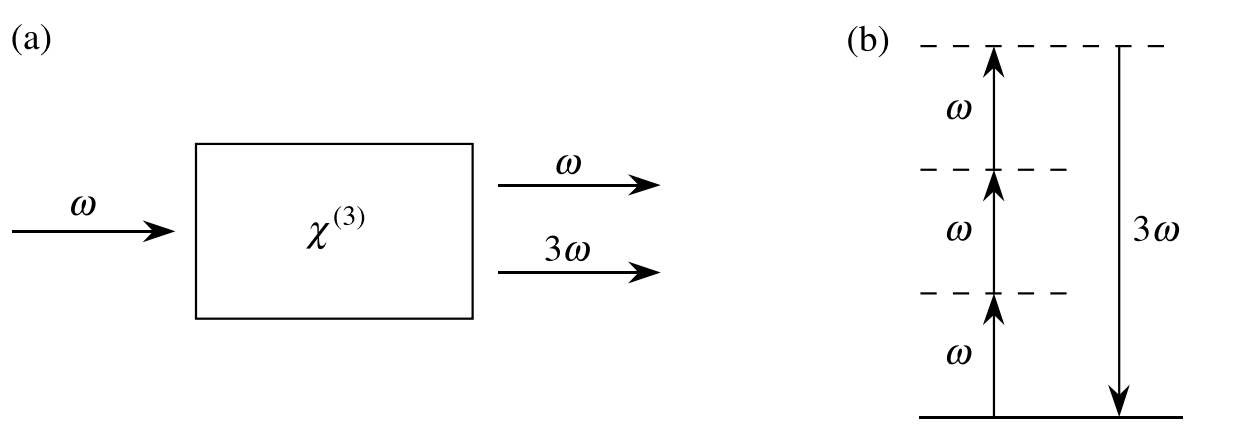
\includegraphics[width=0.95\textwidth]{Images/thg.png}\\
      {\tiny Schematische Darstellung: Drei Photonen $\omega$ erzeugen ein Photon $3\omega$. \figciteweb{Boyd2020}}
  \end{columns}
  \vspace{0.2cm}
  \begin{itemize}
    \item \textbf{Energieerhaltung:} $3\hbar\omega = \hbar(3\omega)$
    \pause
    \item \textbf{Praxis:} THG tritt auch in Flüssigkeiten und Gasen auf, nicht nur in Kristallen
  \end{itemize}
  \note{
    Bei der Drittharmonischen Generation (THG) verschmelzen drei Photonen der Frequenz $\omega$ zu einem Photon mit $3\omega$.\newline
    Im Gegensatz zur SHG ist kein Symmetriebruch nötig: $\chi^{(3)}$ ist in allen Materialien vorhanden, daher kann THG auch in zentrosymmetrischen Medien (z.B. Flüssigkeiten) auftreten.\newline
    Die Formel $P^{(3)}(3\omega) = \varepsilon_0 \chi^{(3)} E(\omega)^3$ beschreibt die Polarisationskomponente bei $3\omega$.\newline
    THG ist meist schwächer als SHG, da der Effekt dritter Ordnung ist.\newline
    Besonders effektiv ist THG an Grenzflächen oder in Bereichen mit Brechungsindexgradienten, z.B. in der THG-Mikroskopie.\newline
    Die schematische Grafik zeigt, wie drei Photonen zu einem Photon mit dreifacher Frequenz verschmelzen.
  }
\end{frame}

\begin{frame}{Nichtlineare Suszeptibilität}
  \begin{columns}[T,onlytextwidth]
    \column{0.48\textwidth}
      \centering
      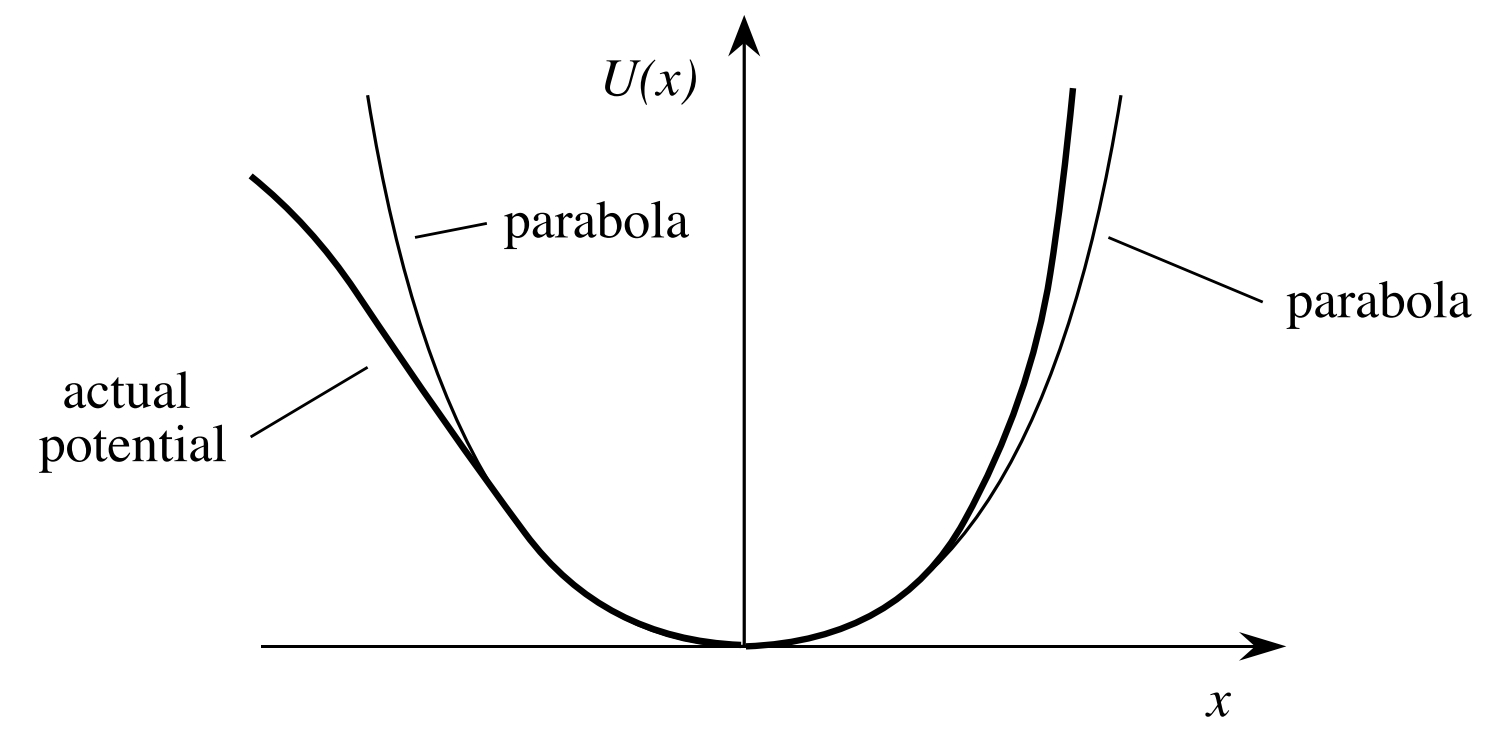
\includegraphics[width=0.7\textwidth]{Images/pot_noncentrosym.png}\\
      {\tiny Nicht-zentrosymmetrisch (\cite{Boyd2020})}
      \begin{itemize}
        \item \textbf{\(\chi^{(2)}\):} Second-order (SHG), nur in nicht-zentrosymmetrischen Materialien
        \pause
        \item \textbf{\(\chi^{(3)}\):} Third-order (THG), in allen Materialien möglich
        \item \textbf{Größenordnungen:} \(\chi^{(2)}\) typ. $10^{-12}$ bis $10^{-8}$ m/V, \(\chi^{(3)}\) noch kleiner
      \end{itemize}
    \column{0.48\textwidth}
      \centering
      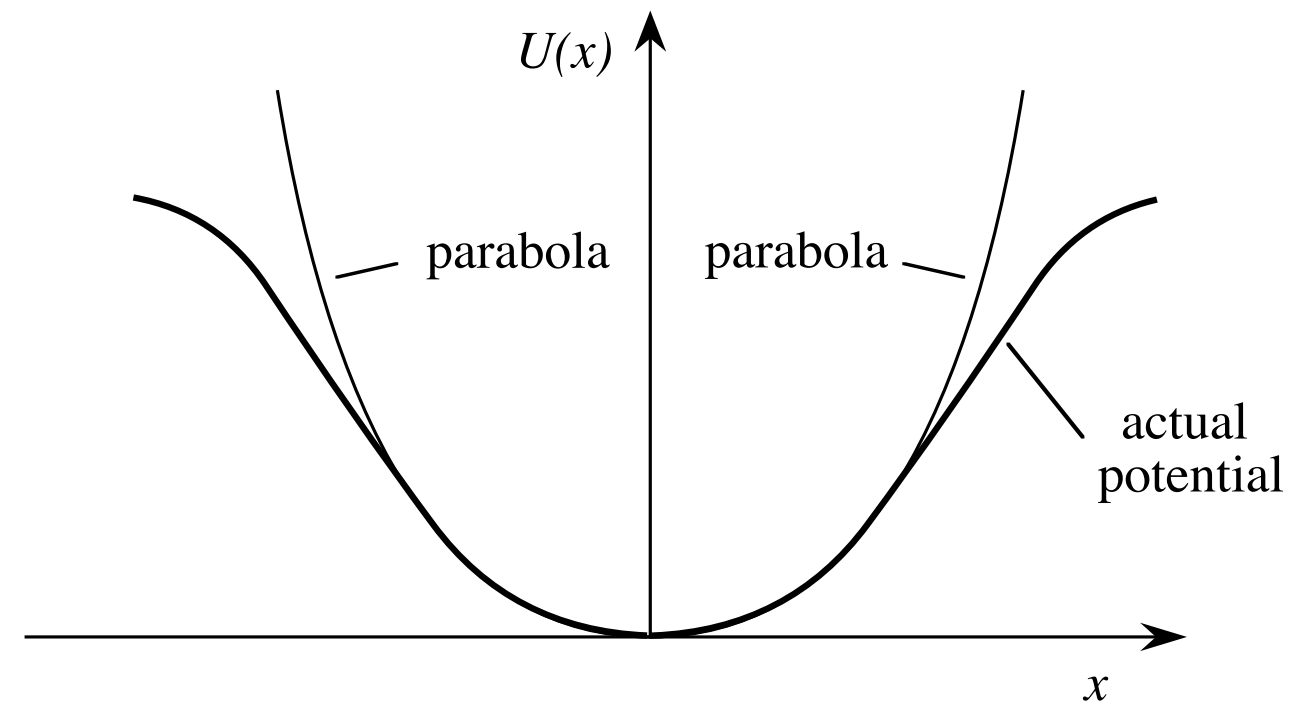
\includegraphics[width=0.7\textwidth]{Images/pot_centrosym.png}\\
      {\tiny Zentrosymmetrisch (\cite{Boyd2020})}
      \begin{itemize}
        \item Symmetrie entscheidet, welche Terme auftreten:
        \pause
        \begin{itemize}
          \item Kein Inversionszentrum: \(\chi^{(2)} \neq 0\), z.B. viele Kristalle
          \item Mit Inversionszentrum: \(\chi^{(2)} = 0\), nur \(\chi^{(3)}\) bleibt
        \end{itemize}
      \end{itemize}
  \end{columns}

  \note{
    Die Folie erklärt, warum nicht alle Materialien für SHG geeignet sind.\newline
    Oben sieht man zwei Potentialtöpfe: links ohne Inversionssymmetrie – hier können gerade und ungerade Terme auftreten, also sowohl \(\chi^{(2)}\) als auch \(\chi^{(3)}\). rechts mit Inversionssymmetrie – hier verschwindet \(\chi^{(2)}\), nur \(\chi^{(3)}\) bleibt.\newline
    Das ist der Grund, warum SHG nur in nicht-zentrosymmetrischen Kristallen beobachtet wird, während THG in allen Materialien möglich ist.\newline
    Die Werte für \(\chi^{(2)}\) sind meist sehr klein, aber in bestimmten Kristallen ausreichend groß für effiziente Frequenzkonversion.\newline
    Symmetrie ist der Schlüssel: Sie entscheidet, welche nichtlinearen Terme auftreten können!
  }
\end{frame}

% --- Folie 8: Phasenanpassung (Phase Matching) ---

\begin{frame}{Phasenanpassung (Phase Matching)}
  \begin{columns}[T,onlytextwidth]
    \column{0.52\textwidth}
      \begin{itemize}
        \item Effiziente SHG/THG: Wellen müssen kohärent bleiben
        \pause
        \item \textbf{Bedingung:} $k(2\omega) = 2k(\omega)$
        \item Ohne Phasenanpassung: geringe Effizienz
        \pause
        \item Kohärenzlänge: Phasenverlust-Abstand
      \end{itemize}
    \column{0.46\textwidth}
      \begin{center}
      \animategraphics[autoplay,loop,width=0.95\columnwidth]{10}{Images/Phase Matching/imperfect}{001}{021}\\[-1mm]{\tiny Animation: Imperfektes Phasenmatching – die erzeugte Welle läuft außer Phase.}
      \end{center}
  \end{columns}
  \note{
    Für effiziente Frequenzkonversion müssen die erzeugte Welle und das Grundsignal phasenkohärent bleiben.\newline
    Ist die Phasenanpassung nicht erfüllt ($k(2\omega) \neq 2k(\omega)$), kommt es zu destruktiver Interferenz und die Effizienz sinkt stark.\newline
    Die Animation zeigt, wie sich bei imperfektem Phasenmatching die erzeugte Welle und das Grundsignal auseinanderlaufen.\newline
    Die Kohärenzlänge ist der Abstand, nach dem die Phasenbeziehung verloren geht.\newline
    Durch Doppelbrechung oder periodische Polung kann die Phasenanpassung gezielt eingestellt werden.
  }
\end{frame}

% --- Folie 8b: Perfektes Phasenmatching (Animation) ---

\begin{frame}{Perfektes Phasenmatching}
  \begin{columns}[T,onlytextwidth]
    \column{0.52\textwidth}
      \begin{itemize}
        \item Phasenbeziehung bleibt erhalten: Wellen laufen synchron
        \pause
        \item Maximale Effizienz der Frequenzkonversion
        \item Erreichbar durch exakte Einstellung von Kristallwinkel, Temperatur oder periodische Polung (QPM)
        \pause
        \item \textbf{QPM:} Die Ausrichtung der elektrischen Dipole wird periodisch umgekehrt (z.B. in Lithiumniobat)
        \item Typ I/II (Birefringenz: Doppelbrechung)
      \end{itemize}
    \column{0.46\textwidth}
      \begin{center}
      \animategraphics[autoplay,loop,width=0.95\columnwidth]{10}{Images/Phase Matching/perfect}{001}{021}\\[-1mm]{\tiny Animation: Perfektes Phasenmatching}
      \end{center}
  \end{columns}
  \note{
    Bei perfektem Phasenmatching bleibt die erzeugte Welle immer in Phase mit dem Grundsignal.\newline
    Dadurch addieren sich die Beiträge konstruktiv und die Effizienz der Frequenzkonversion ist maximal.\newline
    In der Praxis wird dies durch exakte Einstellung des Kristallwinkels, der Temperatur oder durch periodische Polung (QPM) erreicht.\newline
    Die \textbf{Ausrichtung der elektrischen Dipole in einem Material} (meist in nichtlinearen Kristallen wie Lithiumniobat) regelmäßig \textbf{in bestimmten Abständen umgekehrt wird}. Das bedeutet, die Polarisation des Materials wechselt periodisch zwischen zwei entgegengesetzten Richtungen.

  
    Birefringenz bedeutet Doppelbrechung: Ein Material hat unterschiedliche Brechungsindizes für verschiedene Polarisationsrichtungen des Lichts. Das ist wichtig, um Phasenanpassung (Phase Matching) zu erreichen, damit nichtlineare optische Prozesse effizient ablaufen.

Typ I und Typ II beschreiben, wie die Polarisationen der beteiligten Lichtwellen zueinander stehen:
\begin{itemize}
  \item \textbf{Typ I:} Zwei Photonen der gleichen Polarisation (z.B. beide senkrecht) erzeugen ein Photon mit doppelter Frequenz, das die entgegengesetzte Polarisation hat.
  \item \textbf{Typ II:} Zwei Photonen unterschiedlicher Polarisation (z.B. eines senkrecht, eines waagerecht) erzeugen gemeinsam das neue Photon.
\end{itemize}
Zusammengefasst:
Typ I/II (Birefringenz) beschreibt die Art der Polarisation und die Rolle der Doppelbrechung bei nichtlinearen optischen Prozessen in Kristallen.

    Die Animation zeigt, wie bei perfektem Phasenmatching die erzeugte Welle und das Grundsignal synchron laufen.
  }
\end{frame}


\section{Experimenteller Aufbau und Messung}
% --- Folie: Experimenteller Aufbau SHG/THG (Schema) ---



% Folie 9: Experimenteller Aufbau (Schema)
\begin{frame}{Experimenteller Aufbau: SHG/THG}
  \begin{columns}[T,onlytextwidth]
    \column{0.55\textwidth}
      \begin{itemize}
        \item Starke Laserquelle (z.B. Nd:YAG, Ti:Sa, gepulst)
        \item Strahlführung: Polarisation, Fokussierung auf Kristall
        \item Nichtlinearer Kristall (z.B. BBO, KTP, LBO), drehbar für Phasenanpassung
        \item Filter blockiert Grundwelle, lässt SHG/THG durch
        \item Detektion: Photodiode oder Spektrometer
      \end{itemize}
    \column<0->{0.43\textwidth}
      \centering
        \includegraphics<0->[width=0.95\textwidth]{Images/Experimental-setup-measuring-SHG-and-THG-intensity-relative-to-laser-energy.png}\\
        {\tiny Experimenteller Aufbau zur Messung der SHG- und THG-Intensität in Abhängigkeit von der Laserenergie, \figcite{ResearchGate2025}}
  \end{columns}
  \note{
    Für SHG/THG benötigt man eine starke, kohärente Laserquelle (oft gepulst, z.B. Nd:YAG 1064 nm oder Ti:Sa 800 nm).\newline
    Der Strahl wird polarisiert und auf einen kleinen Spot im nichtlinearen Kristall fokussiert, um die Intensität zu erhöhen.\newline
    Typische Kristalle: BBO, KTP, LBO, je nach gewünschter Wellenlänge und Phase-Matching-Bedingung.\newline
    Nach dem Kristall werden Filter eingesetzt, die das Grundsignal blockieren und nur die erzeugte Harmonische durchlassen.\newline
    Die Detektion erfolgt meist mit einer Photodiode oder einem Spektrometer.\newline
    Die Effizienz hängt von Polarisation, Winkel und Temperatur des Kristalls ab.
  }
\end{frame}

% Folie 10: Komponenten und Messung
\begin{frame}{Komponenten und Messung}
  \begin{columns}[T,onlytextwidth]
    \column{0.55\textwidth}
      \begin{itemize}
        \item \textbf{Laser:} Pulsdauer, Wellenlänge, Leistung
        \item \textbf{Kristall:} Material, Dicke, Temperatur, Ausrichtung!
        \item \textbf{Messung:} Intensität der Harmonischen in Abhängigkeit von Polarisation, Winkel, Leistung
        \item Typisch: Quadratische Abhängigkeit für SHG ($I_{SHG} \propto P^2$)
      \end{itemize}
    \column{0.43\textwidth}
      \centering
      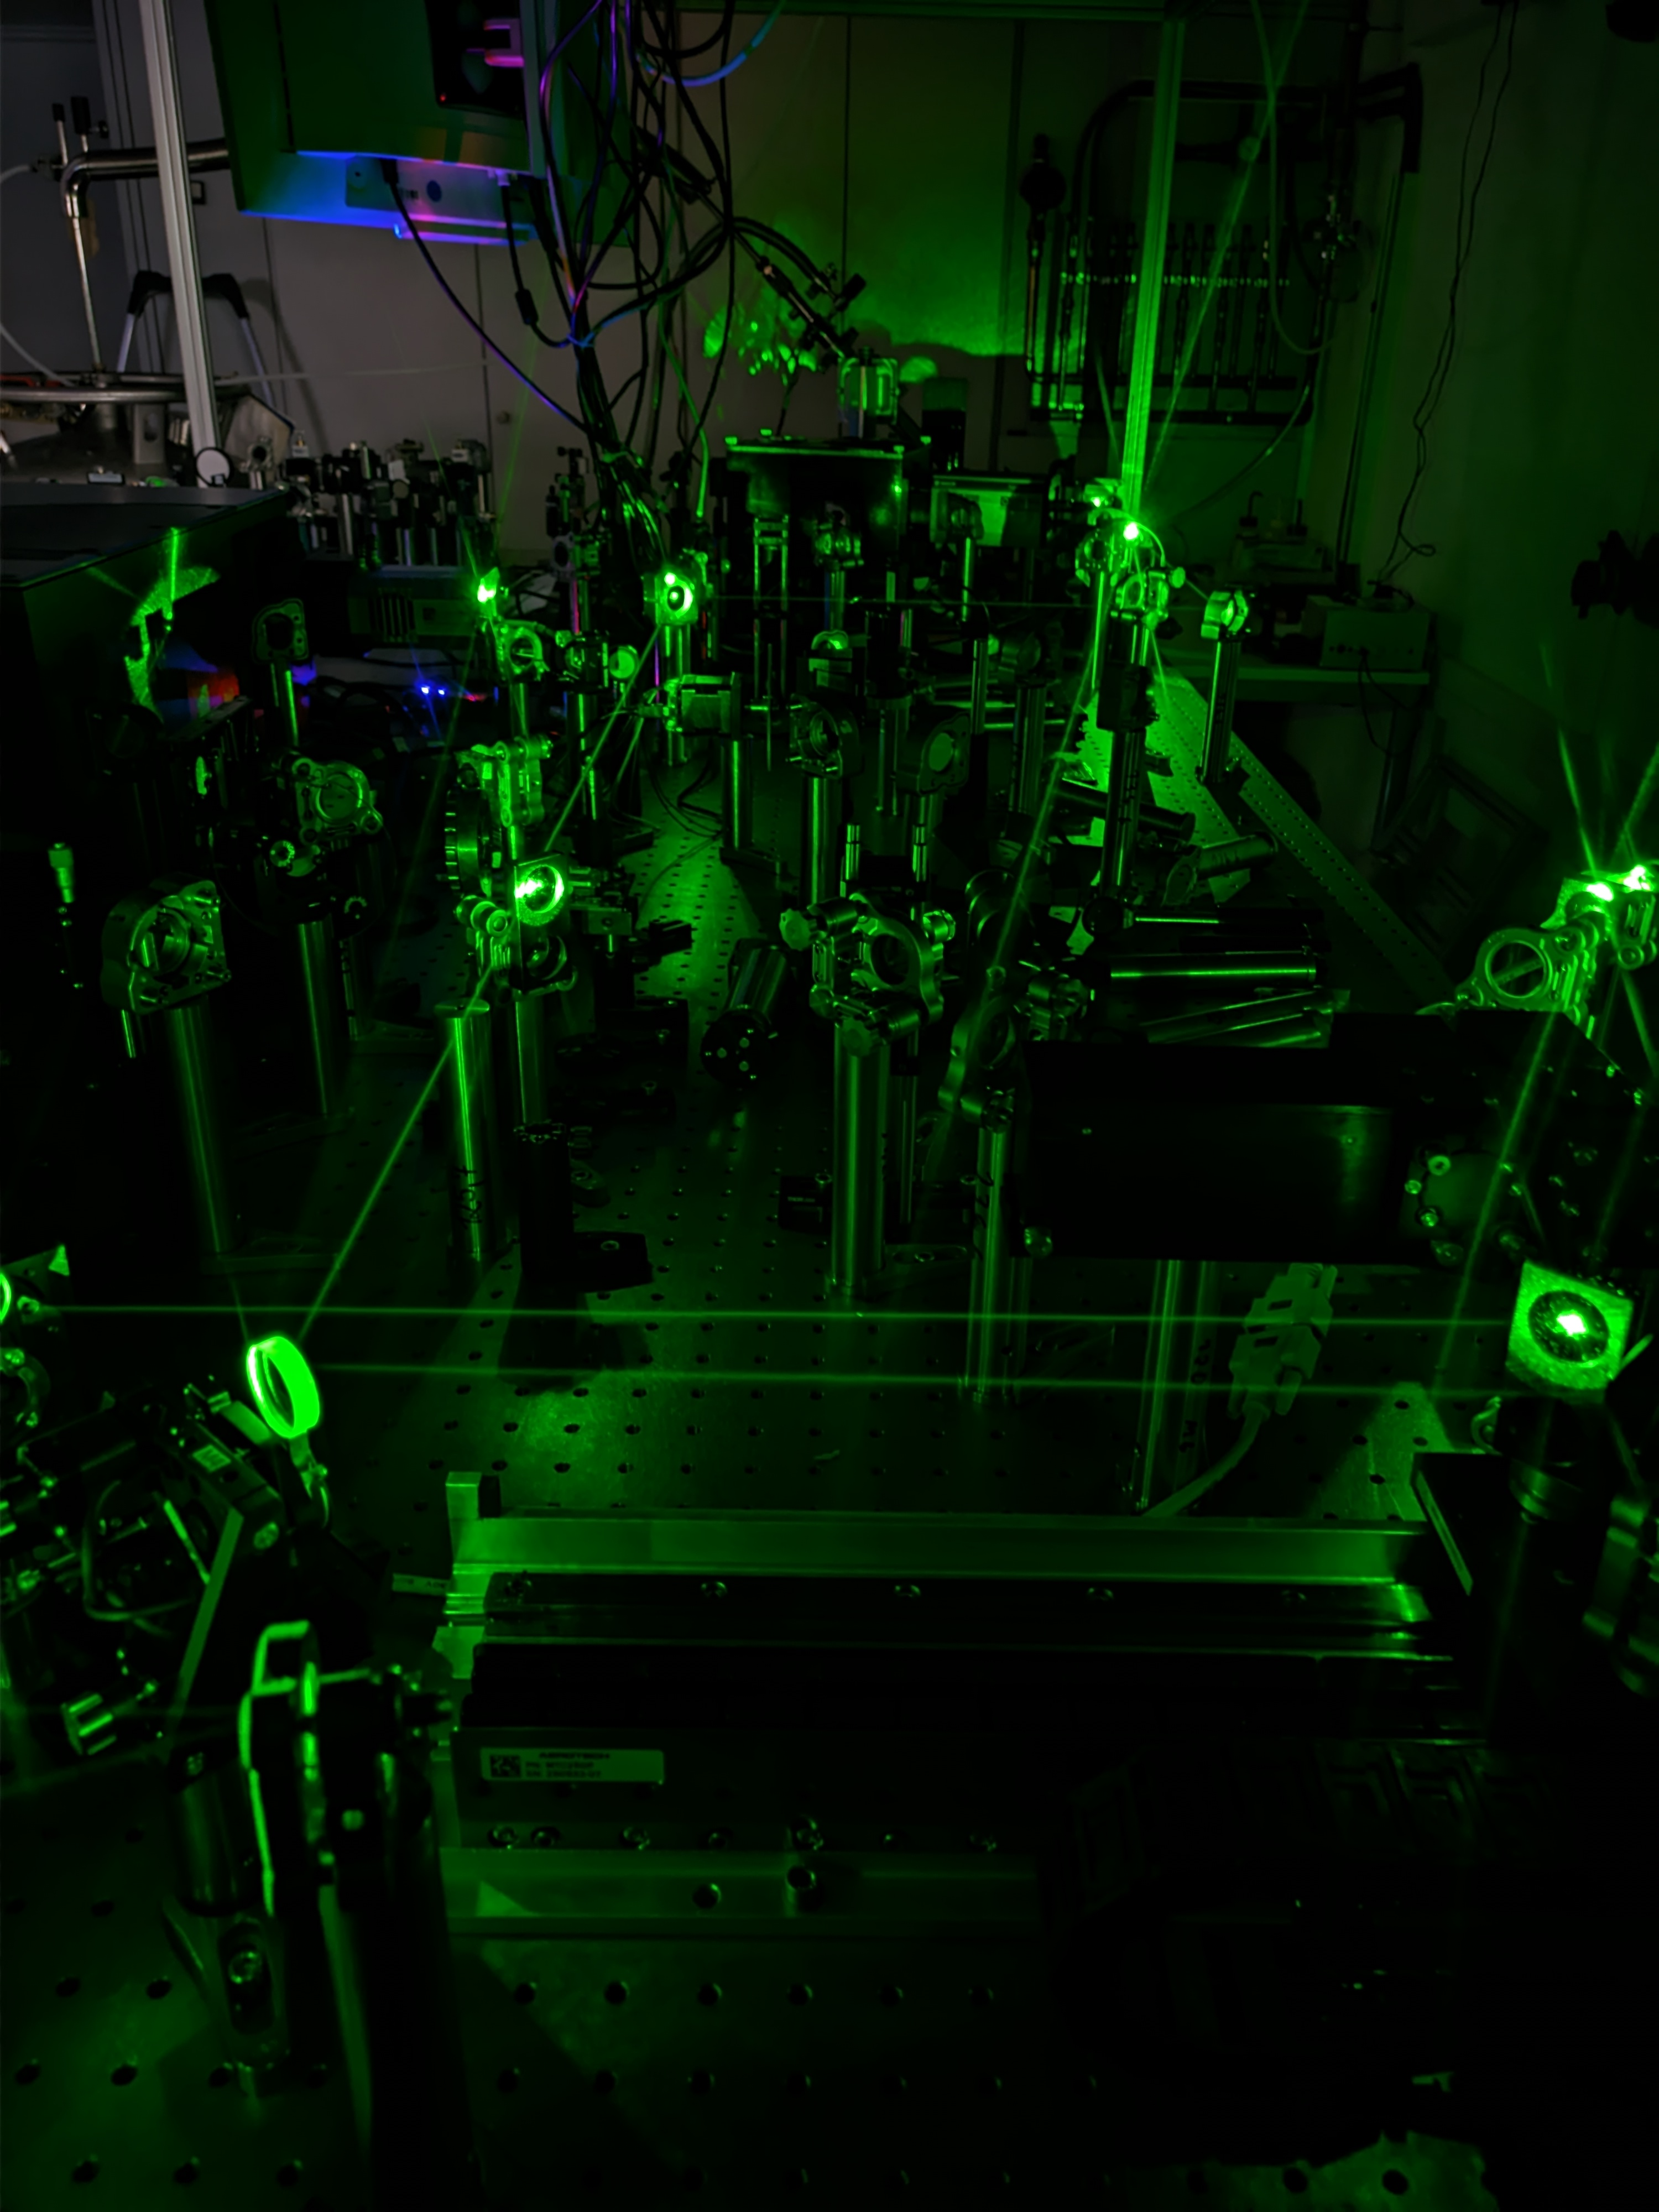
\includegraphics[height=0.8\textheight]{Images/PXL_20250318_131716572.NIGHT.jpg}
      {\figcite{Adamczyk2025}}
  \end{columns}
  \note{
    Die wichtigsten Komponenten sind Laser, Kristall, Strahlführung, Filter und Detektor.\newline
    Die Polarisation und der Winkel des Kristalls werden so eingestellt, dass das Phasenmatching optimal ist.\newline
    Die Intensität der erzeugten Harmonischen wird gemessen und z.B. gegen die Eingangsleistung oder den Kristallwinkel aufgetragen.\newline
    Typisch ist eine quadratische Abhängigkeit der SHG-Intensität von der Eingangsleistung.\newline
    Für THG ist die Abhängigkeit kubisch.\newline
    Die Messung kann mit einem Spektrometer oder einer Photodiode erfolgen.\newline
    Filter sind wichtig, um das Grundsignal zu unterdrücken und nur die Harmonische zu detektieren.
  }
\end{frame}


\section{Anwendungen und Beispiele}
% --- Folie: Anwendungen und Beispiele (SHG/THG) ---

\begin{frame}{Anwendungen und Beispiele: SHG/THG}
  \begin{columns}[T,onlytextwidth]
    \column{0.52\textwidth}
      \begin{itemize}
        \item Grüne Laserpointer (SHG, 532 nm)
        \pause
        \item Oberflächen-/Grenzflächenspektroskopie
        \item SHG-Mikroskopie: z.B. Kollagen, Gewebe
        \pause
        \item THG-Mikroskopie: label-free Imaging
        \item Frequenzkonversion: neue Laserfarben
        \item Materialcharakterisierung ($\chi^{(2)}$, $\chi^{(3)}$)
      \end{itemize}
    \column{0.46\textwidth}
      \centering
      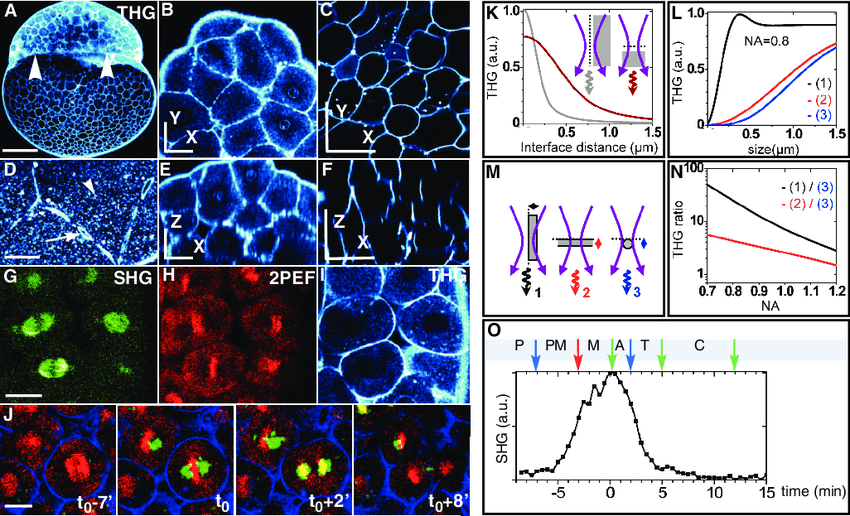
\includegraphics[width=0.98\textwidth]{Images/THG-and-SHG-signals-in-the-zebrafish-embryo-during-cleavage-stages-A-Sagittal-THG.png}\\
      {\tiny SHG/THG-Mikroskopie am Zebrafisch-Embryo\figciteweb{ResearchGateZebrafish2009}}
  \end{columns}
  \note{
    \textbf{SHG-Anwendungen:}
    \begin{itemize}
      \item Grüne Laserpointer nutzen SHG, um aus einem IR-Laser (1064 nm) sichtbares Licht (532 nm) zu erzeugen.
      \item In der Oberflächen- und Grenzflächenspektroskopie ist SHG besonders sensitiv, da nur nicht-zentrosymmetrische Bereiche (z.B. Oberflächen, Grenzflächen) ein Signal liefern. So lassen sich z.B. Monolagen oder Adsorbate an Oberflächen untersuchen.
      \item SHG-Mikroskopie wird in der Biologie genutzt, um Strukturen wie Kollagenfasern sichtbar zu machen. Da SHG nur in bestimmten Geweben auftritt, ist die Bildgebung sehr selektiv und benötigt keine Fluoreszenzmarker.
    \end{itemize}
    \textbf{THG-Anwendungen:}
    \begin{itemize}
      \item THG-Mikroskopie ermöglicht label-freie Bildgebung, da das Signal an Grenzflächen und Brechungsindex-Übergängen entsteht (z.B. Zellmembranen, Lipidtröpfchen).
      \item In der Materialcharakterisierung kann über die Intensität der THG das $\chi^{(3)}$ eines Materials bestimmt werden.
    \end{itemize}
    \textbf{Beispielbild Zebrafisch-Embryo:}
    \begin{itemize}
      \item Gezeigt werden THG- und SHG-Signale im Zebrafisch-Embryo während der Furchungsstadien.
      \item THG hebt Grenzflächen wie das Dotter-Blastoderm-Interface, Zellgrenzen und Organellen hervor (z.B. weiße Pfeilspitzen, verschiedene NA und Projektionen).
      \item SHG macht Strukturen wie Kollagen oder die Dynamik der Zellteilung sichtbar (z.B. Intensitätsverlauf während Mitose).
      \item Die Bildgebung ist komplett label-free und nutzt unterschiedliche numerische Aperturen (NA) für verschiedene Details.
      \item Die Kombination von SHG, THG und 2-Photonen-Fluoreszenz (2PEF) erlaubt die Rekonstruktion von Zellgrenzen, Vesikeln und Membranen in hoher Auflösung.
    \end{itemize}
    \textbf{Allgemein:}
    \begin{itemize}
      \item Frequenzkonversion (SHG/THG) erweitert das Farbspektrum von Lasern und ist für viele Anwendungen in der Spektroskopie, Medizin und Mikroskopie essenziell.
    \end{itemize}
  }
\end{frame}

% --- Folie: Zusammenfassung und Ausblick ---

\begin{frame}{Zusammenfassung und Ausblick}
  \begin{itemize}
    \item SHG: 2$\omega$ ($\chi^{(2)}$) – nur in nichtzentrosymmetrischen Medien
    \pause
    \item THG: 3$\omega$ ($\chi^{(3)}$) – überall möglich
    \item Effizient nur mit starken Lasern + Phasenanpassung
    \pause
    \item Anwendungen: Laser (sichtbar), Mikroskopie, Spektroskopie
    \item Ausblick: Höhere Harmonische (z.B. HHG) möglich
  \end{itemize}
  \note{
    \textbf{Kernpunkte:}
    \begin{itemize}
      \item Nichtlineare Optik ermöglicht die Erzeugung neuer Lichtfrequenzen durch Prozesse wie SHG (Frequenzverdopplung) und THG (Frequenzverdreifachung).
      \item SHG ist nur in nicht-zentrosymmetrischen Materialien möglich, da $\chi^{(2)}$ dort ungleich null ist. THG kann in allen Medien auftreten, da $\chi^{(3)}$ immer existiert.
      \item Für eine effiziente Umsetzung sind starke, meist gepulste Laser und exaktes Phasenmatching nötig.
      \item Anwendungen reichen von der Erzeugung sichtbaren Lichts (z.B. grüne Laserpointer) über die nichtlineare Mikroskopie (SHG/THG Imaging) bis zur Materialanalyse und Spektroskopie.
      \item Die Frequenzkonversion erweitert das nutzbare Spektrum von Lasern und ist für viele moderne Technologien essenziell.
    \end{itemize}
    \textbf{Ausblick:}
    \begin{itemize}
      \item Neben SHG und THG gibt es noch höhere Harmonische (z.B. HHG – High Harmonic Generation), die aber zunehmend komplexere Bedingungen und noch höhere Intensitäten erfordern.
      \item Die Forschung an neuen Materialien und Techniken (z.B. Quasi-Phasenmatching, Nanostrukturen) eröffnet ständig neue Anwendungen.
    \end{itemize}
    Vielen Dank für Ihre Aufmerksamkeit!\newline
    Fragen?
  }
\end{frame}

 % Thank You Slide
    \begin{frame}{Vielen Dank der Aufmerksamkeit!}
      \begin{center}
          \Huge Fragen?
      \end{center}
  \end{frame}

% Black slide
\begin{frame}<handout:0>[plain, noframenumbering]
  \begin{tikzpicture}[remember picture, overlay]
      \fill[black] (current page.south west) rectangle (current page.north east);
  \end{tikzpicture}
\end{frame}

% --- Anhang: SHG vs. Zweiphotonenabsorption (TPA) ---

\begin{frame}[noframenumbering]{SHG ist nicht gleich Zweiphotonenabsorption (TPA)}
  \begin{columns}[T,onlytextwidth]
    \column{0.48\textwidth}
      \begin{itemize}
        \item SHG: Kohärenter, \textbf{parametrischer} Prozess
        \item TPA: Nichtkohärent, \textbf{nichtparametrisch}
        \item SHG: Virtuelle Zustände, keine echte Anregung
        \item TPA: Reale Zwischenzustände, echte Absorption
        \item SHG: Signal bei $2\omega$ messen
        \item TPA: Transmission bei $\omega$ messen
      \end{itemize}
    \column{0.56\textwidth}
      \centering
      \only<1>{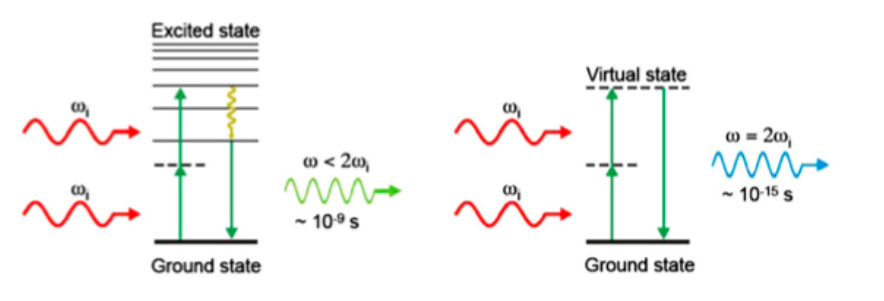
\includegraphics[width=0.98\textwidth]{Images/shg vs tpa.png}\\[-1mm]{\tiny SHG vs. TPA: Prinzipdarstellung, \figcite{Zhang2020}}}
      \only<2>{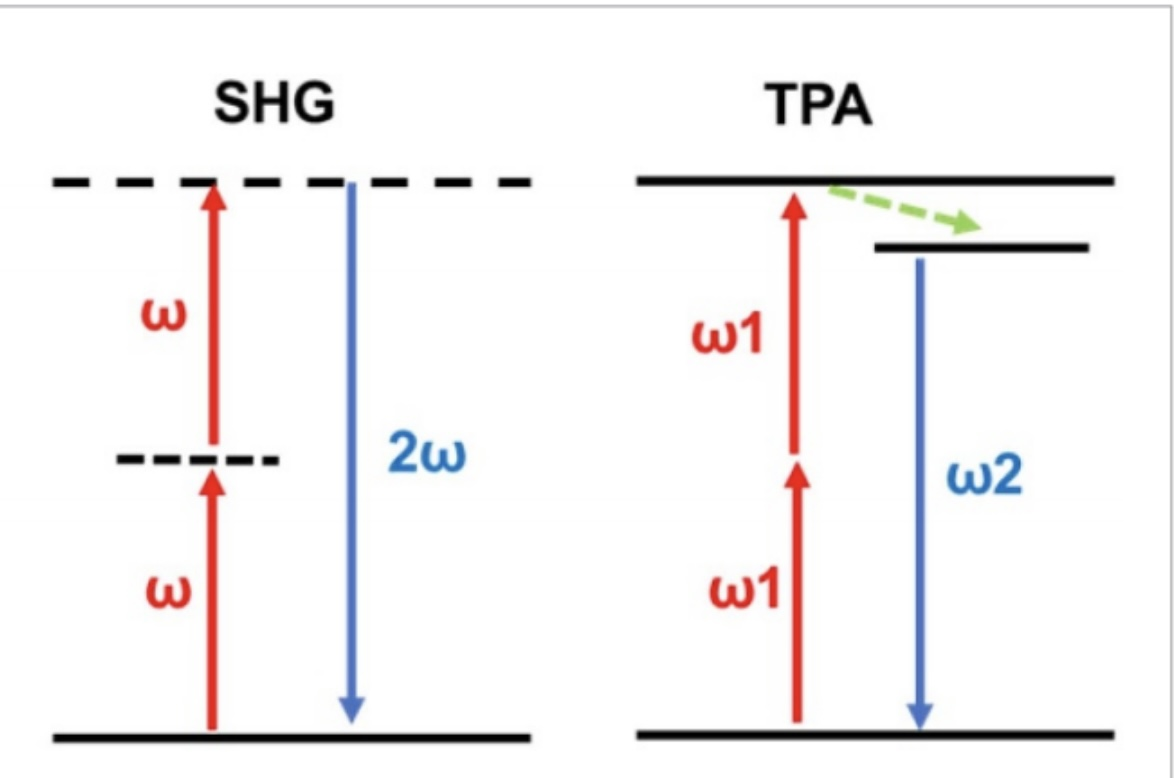
\includegraphics[width=0.8\textwidth]{Images/40EB55CB-B2EC-4C0E-BFFB-EA95D7FE419A.jpeg}\\[-1mm]{\tiny Energieniveaus: SHG (oben), TPA (unten) \cite{Bhattacharya2012}}}
  \end{columns}
  \note{
    \textbf{SHG (Second Harmonic Generation):}
    \begin{itemize}
      \item Zwei Photonen werden im nichtzentrosymmetrischen Medium kohärent zu einem Photon mit doppelter Frequenz kombiniert.
      \item Die Elektronen werden dabei nur in virtuelle Zustände angeregt – es findet keine echte Absorption statt.
      \item SHG ist ein \textbf{parametrischer} Prozess: Energie und Impuls werden erhalten, aber es gibt keinen Netto-Übergang zwischen echten Zuständen.
      \item Das Signal wird bei $2\omega$ detektiert.
    \end{itemize}
    \textbf{TPA (Zweiphotonenabsorption):}
    \begin{itemize}
      \item Zwei Photonen werden gleichzeitig absorbiert und heben das Elektron in einen echten angeregten Zustand.
      \item Es findet echte Absorption statt, gefolgt ggf. von Relaxation oder Fluoreszenz.
      \item TPA ist ein \textbf{nichtparametrischer} Prozess und drittordnungs-nonlinear ($\chi^{(3)}$).
      \item Das Signal wird als Änderung der Transmission bei $\omega$ gemessen.
    \end{itemize}
    \textbf{Weitere Unterschiede:}
    \begin{itemize}
      \item SHG ist nur in nichtzentrosymmetrischen Medien möglich ($\chi^{(2)}$), TPA überall ($\chi^{(3)}$).
      \item SHG ist kohärent (phasengekoppelt), TPA nicht.
      \item In der Praxis: SHG erzeugt Licht bei neuer Frequenz, TPA führt zu Absorption und ggf. Fluoreszenz.
    \end{itemize}
    \textbf{Bilderklärung:}
    \begin{itemize}
      \item Erstes Bild: Schematischer Vergleich der Prozesse (SHG: Wellenüberlagerung, TPA: echte Anregung).
      \item Zweites Bild: Energieniveaus – oben SHG (virtuelle Zustände), unten TPA (reale Zustände).
      \item Durch Klicken wird das zweite Bild eingeblendet.
    \end{itemize}
    \textbf{Literatur:} Robert Boyd, Nonlinear Optics.
  }
\end{frame}

% --- Anhang: Sequential THG und High Harmonic Generation (HHG) ---

\begin{frame}[noframenumbering]{Sequential THG und High Harmonic Generation (HHG)}
  \begin{columns}[T,onlytextwidth]
    \column{0.48\textwidth}
      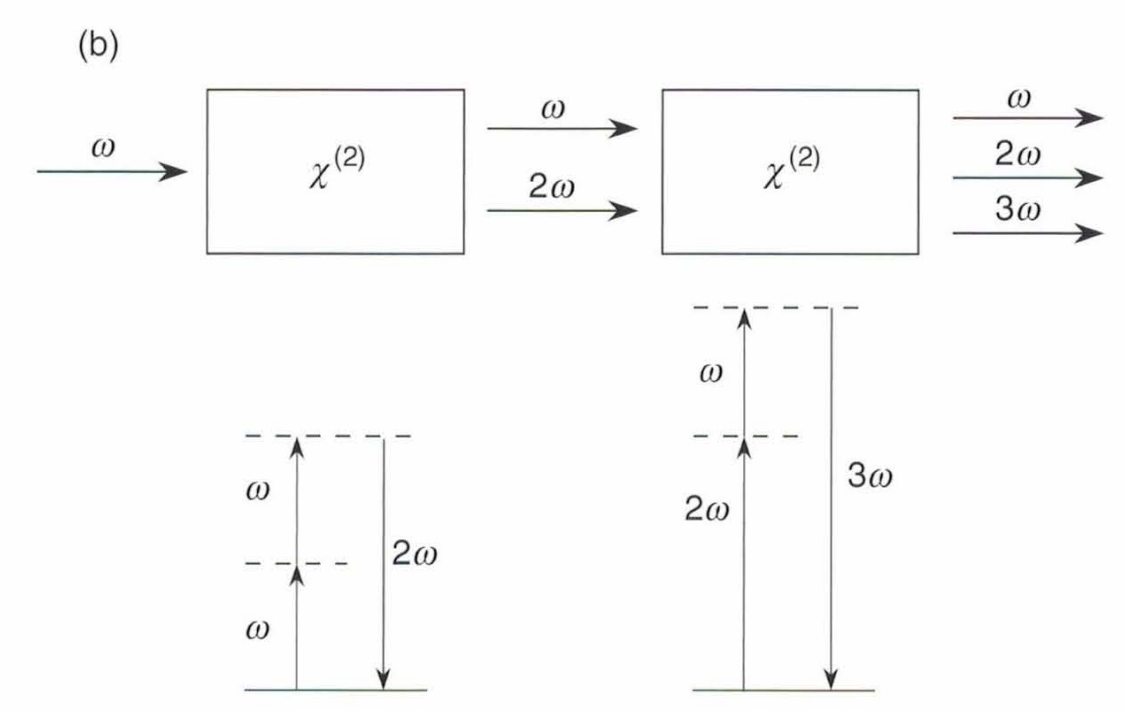
\includegraphics[width=0.98\textwidth]{Images/seq_thg.png}\\[-1mm]{\tiny Sequential THG \figcite{Boyd2020}}
    \column{0.48\textwidth}
      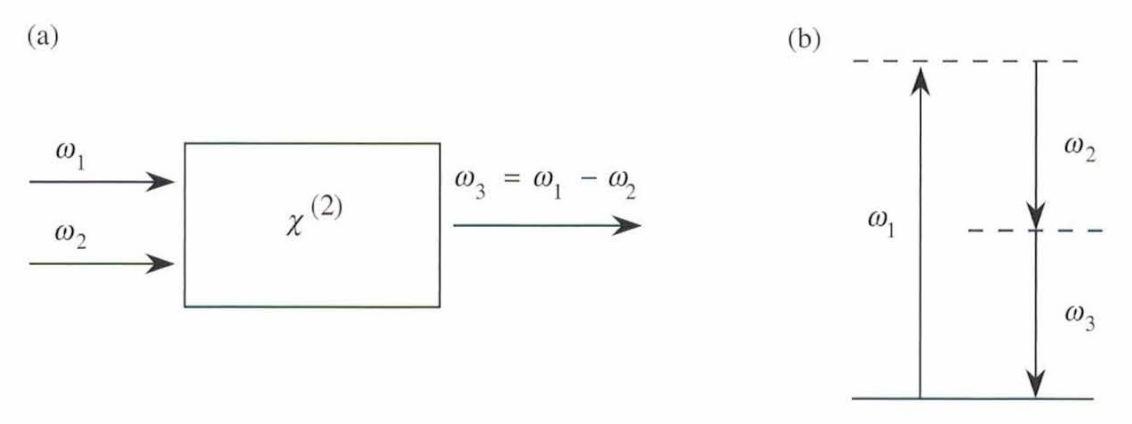
\includegraphics[width=0.98\textwidth]{Images/hhg.png}\\[-1mm]{\tiny High Harmonic Generation \figcite{Boyd2020}}
  \end{columns}
  \vspace{0.2cm}
  \begin{itemize}
    \item Sequential THG: Mehrstufige Frequenzkonversion (z.B. $\omega \rightarrow 2\omega \rightarrow 3\omega$)
    \item HHG: Erzeugung sehr hoher Harmonischer (bis XUV), starker Laser nötig
    \item HHG: Nichtlinear, nichtperturbativ, Tunnelionisation
  \end{itemize}
  \note{
    \textbf{Sequential THG:}
    \begin{itemize}
      \item Die dritte Harmonische kann auch sequentiell erzeugt werden: Erst SHG ($\omega \rightarrow 2\omega$), dann Sum-Frequenz-Generation ($\omega + 2\omega \rightarrow 3\omega$).
      \item Vorteil: Effizienter in manchen Materialien, da jede Stufe optimiert werden kann.
      \item Bild links: Schematische Darstellung der sequentiellen Prozesse.
    \end{itemize}
    \textbf{High Harmonic Generation (HHG):}
    \begin{itemize}
      \item Bei sehr hohen Intensitäten (starke Femtosekundenlaser) können noch viel höhere Harmonische (bis ins Extreme UV) erzeugt werden.
      \item HHG ist ein nichtperturbativer Prozess: Das Elektron wird durch das starke Feld ionisiert, beschleunigt und rekombiniert, wobei ein hochenergetisches Photon emittiert wird.
      \item Typisch für Attosekunden-Pulsquellen und moderne Laserspektroskopie.
      \item Bild rechts: Schematische Darstellung des HHG-Prozesses.
    \end{itemize}
    \textbf{Quellen:} Boyd, Nonlinear Optics.
  }
\end{frame}

% --- Anhang: Sum-Frequenz- und Differenz-Frequenz-Generation (SFG/DFG) ---

\begin{frame}[noframenumbering]{Sum-Frequenz- und Differenz-Frequenz-Generation (SFG/DFG)}
  \begin{columns}[T,onlytextwidth]
    \column{0.48\textwidth}
      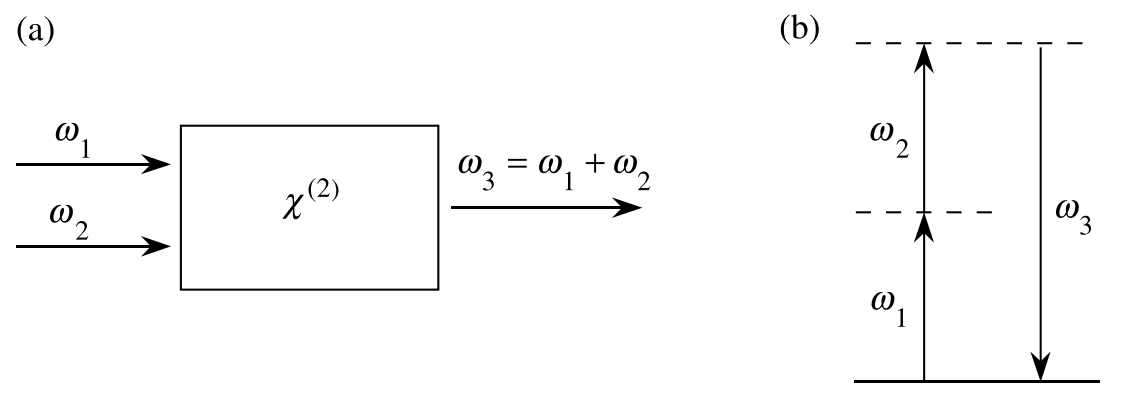
\includegraphics[width=0.98\textwidth]{Images/sum-freq.png}\\[-1mm]{\tiny Sum-Frequenz-Generation (SFG) \figcite{Boyd2020}}
    \column{0.48\textwidth}
      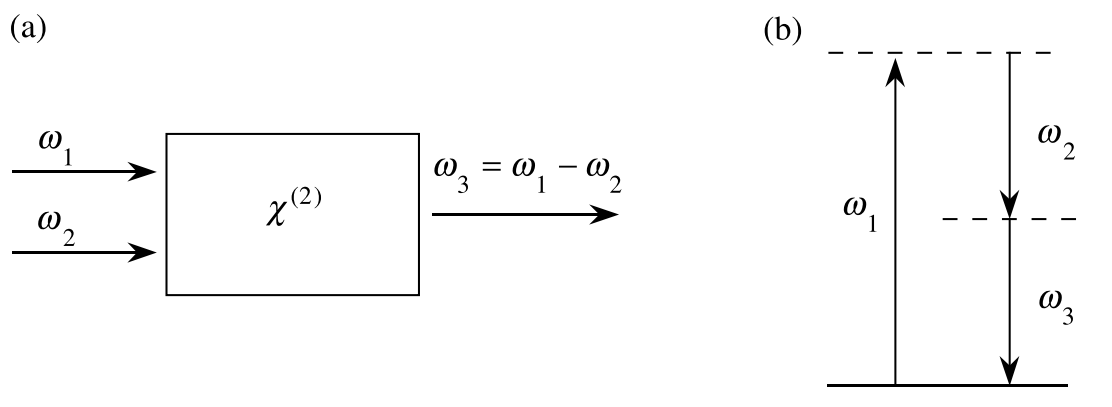
\includegraphics[width=0.98\textwidth]{Images/diff-freq.png}\\[-1mm]{\tiny Differenz-Frequenz-Generation (DFG) \figcite{Boyd2020}}
  \end{columns}
  \vspace{0.2cm}
  \begin{itemize}
    \item \textbf{SFG:} Zwei Photonen unterschiedlicher Frequenz ($\omega_1$, $\omega_2$) erzeugen ein Photon mit $\omega_3 = \omega_1 + \omega_2$
    \item \textbf{DFG:} Zwei Photonen ($\omega_1$, $\omega_2$) erzeugen ein Photon mit $\omega_3 = |\omega_1 - \omega_2|$
    \item Beide Prozesse: Nichtlinear ($\chi^{(2)}$), benötigen starke Felder und Phasenanpassung
  \end{itemize}
  \note{
    \textbf{Sum-Frequenz-Generation (SFG):}
    \begin{itemize}
      \item Zwei Photonen unterschiedlicher Frequenz ($\omega_1$, $\omega_2$) werden im nichtlinearen Medium zu einem Photon mit der Summe der Frequenzen ($\omega_3 = \omega_1 + \omega_2$) kombiniert.
      \item SFG wird z.B. zur Erzeugung neuer Laserwellenlängen genutzt, wenn die gewünschte Frequenz nicht direkt verfügbar ist.
      \item Bild links: Schematische Darstellung des SFG-Prozesses.
    \end{itemize}
    \textbf{Differenz-Frequenz-Generation (DFG):}
    \begin{itemize}
      \item Zwei Photonen ($\omega_1$, $\omega_2$) erzeugen ein Photon mit der Differenzfrequenz ($\omega_3 = |\omega_1 - \omega_2|$).
      \item DFG wird z.B. zur Erzeugung von Terahertz- oder Infrarotstrahlung verwendet.
      \item Bild rechts: Schematische Darstellung des DFG-Prozesses.
    \end{itemize}
    \textbf{Beide Prozesse:}
    \begin{itemize}
      \item SFG und DFG sind wie SHG Prozesse zweiter Ordnung ($\chi^{(2)}$) und benötigen starke Felder sowie exaktes Phasenmatching.
      \item Sie sind wichtige Werkzeuge zur Erweiterung des spektralen Bereichs von Lasern und für die nichtlineare Spektroskopie.
    \end{itemize}
    \textbf{Quelle:} Boyd, Nonlinear Optics.
  }
\end{frame}

\begin{frame}[noframenumbering]{SHG: Propagation und Oberflächen-SHG}
  \begin{columns}[T,onlytextwidth]
    \column{0.48\textwidth}
      \centering
      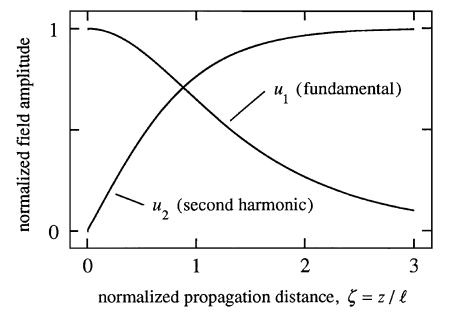
\includegraphics[height=0.28\textheight]{Images/propagation distance.png}\\
      {\tiny SHG-Intensität in Abhängigkeit von der Propagationsdistanz. \figcite{Boyd2020}}
      \vspace{0.4cm}

      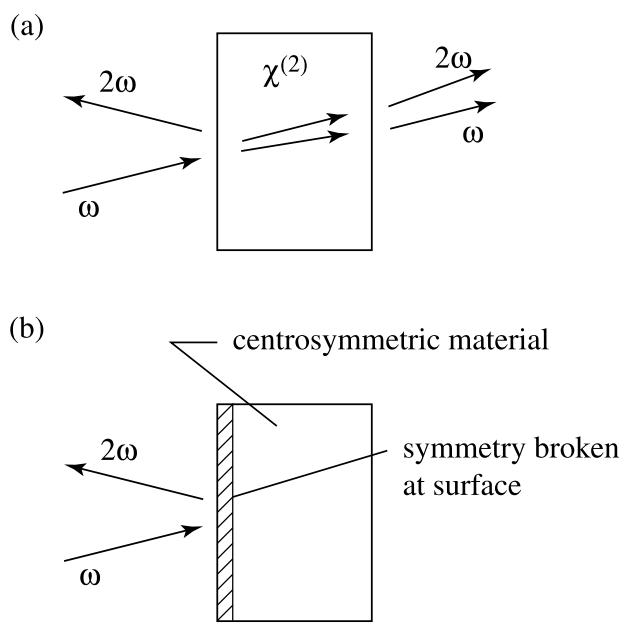
\includegraphics[height=0.46\textheight]{Images/surface-shg.png}\\
      {\tiny Schematische Darstellung: Oberflächen-SHG. \figcite{Boyd2020}}

    \column{0.48\textwidth}
      \centering
      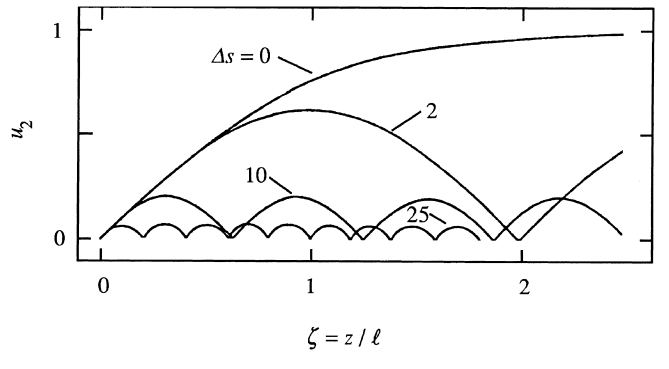
\includegraphics[height=0.28\textheight]{Images/wavevector mismatch.png}\\
      {\tiny Emission bei schlechtem Phase-Matching $\Delta k$. \figcite{Boyd2020}}
      \vspace{0.4cm}

      \includegraphics[height=0.5\textheight]{Images/PXL_20250227_153205340.jpg}
      {\tiny \figciteweb{Adamczyk2025}}
      \vspace{0.3cm}
  \end{columns}

  \note{
    Die Abbildungen zeigen typische Aspekte der SHG: Links oben die Intensitätsentwicklung entlang der Propagationsstrecke, darunter die Rolle des Wellenvektormismatchs an Oberflächen. Rechts oben die Definition der Kohärenzlänge, darunter ein Schema für Oberflächen-SHG. Alle Bilder aus Boyd, Nonlinear Optics.
  }
\end{frame}

    % Bibliography    
  \begin{frame}[allowframebreaks, noframenumbering, plain]{Literaturverzeichnis}
   \printbibliography
    \end{frame}

\end{document}
